\section{Detección de Patologías en Pulmones con Rayos X}

Diferentes trabajos se han limitado a clasificar \textit{COVID-2019} y \textit{no COVID-2019} (o
neumonía), es por ello que durante este trabajo desarrollamos un sistemas más completo para {
distinguir 15 diferentes enfermedades pulmonares.

We experimentally evaluated the proposed model for diagnosis of the 15 lung diseases, obtaining
competitive results, in particular for COVID-19. We compare it with several recent works that classify
14 pathologies (excluding COVID-19); the results in terms of Area Under Curve of the Receiver Operator
Characteristic show a competitive performance of the proposed method for the ChestX-Ray14 pathologies
and a remarkable performance in detecting pneumonia from COVID-19.

In this work we developed a deep learning method that uses as BKN the ResNet50 network, a wildly
used network by the community for implementing different image analysis methods. We extend the
ChestX-Ray14 dataset by including radiographs of Normal and COVID-19 infected patients. Our training
consists of three stages, DTL from the ResNet50 pretrained in ImageNet by replacing the classification
stage by a 15 pathologies classifier, a fine-tuning stage to adjust the last convolutional layers,
and a full-tuning stage that adjusts the weights of the entire network. We demonstrate with experiments
that our proposal is able to preserve the performance of the state of the art 14 pathologies classifiers,
and at the same time achieve the state of the art performance of binaries classifiers for COVID-19.
Additionally, in order to demonstrate that the proposed model can be easily extended for other
pathologies, we implemented a binary classifier for Tuberculosis, a particular bacterial pneumonia
\cite{stirenko2018chest}, with performance comparable to \emph{ad hoc} deep learning models
\cite{puttagunta2021detection}.

in our work we also use the ChestX database \cite{wang2017chestx} and include X-rays of COVID-19 and
healthy (images of persons without known lung diseases) classes. The ChestX-ray14 contains 112,120
frontal-view (both postero-anterior and antero-posterior) chest radiographs of 30,805 unique patients.
Each image is annotated with 14 thoracic pathology labels. We enriched such a dataset with COVID-19,
pneumonia, and healthy chest radiographs. Table~\ref{table_dataset} summarizes the composition of
the dataset used in our work.

\begin{table}[!ht]
    \centering
    \begin{tabular}{| r |l | c | c | c |}
     \hline
     Class & Disease & Source & Train & Test  \\
     \hline\hline
     1  & Cardiomegaly       & 1 & 5897  & 1069 \\
     2  & Emphysema          & 1 & 3496  & 1093 \\
     3  & Effusion           & 1 & 13737 & 4658 \\
     4  & Hernia             & 1 & 4470  & 86   \\
     5  & Infiltration       & 1 & 17122 & 6112 \\
     6  & Mass               & 1 & 7862  & 1748 \\
     7  & Nodule             & 1 & 9250  & 1623 \\
     8  & Atelectasis        & 1 & 13762 & 3279 \\
     9  & Pneumothorax       & 1 & 6303  & 2665 \\
     10 & Pleural-Thick.     & 1 & 8022  & 1143 \\
     11 & Pneumonia          & 1 & 6031  & 555  \\
     12 & Fibrosis           & 1 & 9072  & 435  \\
     13 & Edema              & 1 & 6953  & 925  \\
     14 & Consolidation      & 1 & 9796  & 1815 \\
     ---&  Healthy           & 1 & 35645 & 9861 \\
     \hline
     11 & Pneumonia          & 2 & 5475  & 594  \\
     15 & COVID-19           & 2 & 2873  & 1904 \\
     ---&  Healthy           & 2 & 8661  & 1926 \\
     \hline
    \end{tabular}
    \caption{Number of chest radiography's per case in the dataset. Sources (DS): (1) ChestX-ray14,
             (2) Internet datasets compilation. Pleural-Thick. means Pleural-Thickening.}
    \label{table_dataset}
\end{table}

\subsubsection{Data Relabelling}
\label{ssec_relabelling}

In order to train our model, we use the relabelled version of the ChestX-ray14 database proposed by
the authors of CheXNet \cite{rajpurkar2018deep}.  According to \cite{rajpurkar2018deep}, the
relabelled data allows to improve the training process significantly. Such relabelling consists of
training multiple times a  neural network with the original training data set and keeping those
models with the best accuracy on the original validation set. Then, the predictions of the individual
models are averaged, and a binary detector of each pathology is computed by using a threshold that
maximizes the F1-score in all the pathologies (see Section~\ref{sec_metrics} for the F1-score
definition). Finally, each training and test datum is relabeled as positive for pathology, if it was
initially labeled as positive or the ensemble prediction is positive. However,  we define the train,
validation, and test data sets according to the original problem; \emph{i.e.}, for the original list and
only use the new labels in the training stage. Thus, we report two results: the first one on the
original test dataset and, just for reference,  with the updated labels in the Appendix.

\subsubsection{Data Preprocessing}

We keep as simple as possible the preprocessing of the radiography, we only perform a histogram
equalization and resize the data to $1024 \times 1024$ pixels.

La datos de entrada son imágenes de 1024
columnas y 1024 filas con 3 canales idénticos. Siguiente la propuesta de \textit{CheXNet}, se hace uso
de multiples funciones de perdida tipo \textit{Binary Cross-Entropy} con distintos pesos
para solventar el desbalanceamiento de clases.

\begin{equation} \label{eq:loss}
    L(\hat y, y) = \sum_{c=0}^{15} \left[ w_c^{(p)} y_c \log \hat y_c  + w_c^{(n)}  (1-y_c) \log  (1- \hat y_c)  \right],
\end{equation}

donde $y$ es el vector de etiquetas reales, $\hat y$ es el vector de etiquetas predichas,
$w_c^{(p)}$ y $w_c^{(n)}$ son los pesos para los casos positivos y negativos de cada clase $c$
respectivamente. Dichos pesos son calculados como sigue:

\begin{equation}\label{eq:weights}
    w_c^{(n)} = \frac{n_c}{N} \;\;\;\;\text{and}\;\;\;\;   w_c^{(p)} = 1-  w_c^{(n)};
\end{equation}

donde $N$ es el tamaño del conjunto de datos, y $n_c$ el número de imágenes radiográficas con
etiquetas $c$ (el número elementos del vector de la $c$-ésima clase iguales a 1). Nótese que los
pesos son inversamente proporcional al número de casos en la clase.


\section{Arquitecturas usadas}
\subsection{Vision Transformers}
\subsection{ViT con cabezas de atención Flexibles}

\section{Alternativa: CNN y Transfer Learning}

El modelo desarrollado es construido tomando \textit{CheXNet} como referencia
\cite{rajpurkar2018deep}, el cual clasifica entre 14 enfermedades
usando el conjunto de datos \textit{ChestX-Ray14} \cite{wang2017chestx}. El modelo propuesto es
construido desde cero y extiende la propuesta de \textit{CheXNet} para incluir la clasificación de
imágenes con \textit{COVID-19}.

\textit{CheXNet} es un modelo basado en redes neuronales para detectar la presencia de 14 diferentes
enfermedades de pulmón. \textit{CheXNet} Usas imagenes de Rayos X de vista frontal como entrada y
un modelo convolucional pre-entrenado como backbone \cite{rajpurkar2018deep}. El modelo backbone usado
por \textit{CheXNet} es la red \textit{DenseNet121} \cite{huang2017densely} que contiene 121 capas
convolucionales entrenadas con la base de datos de \textit{ImageNet} \cite{ILSVRC15}. Las imágenes
analizadas por el modelo pueden corresponder a vistas anterior-posterior o posterior-anterior. La
implementación de Transferencia de Conocimiento es lograda removiendo la etapa de clasificación
(formada por capas densas) mientras que la etapa convolucional previa permanece intacta funcionando
como un extractor de características. Posteriormente, una nueva etapa de clasificación construida
para la detección de 14 enfermedades es colocada en su lugar. Finalmente, la nueva red compuesta
es entrenada usando la base de datos \textit{ChestX-Ray14} manteniendo fijos los pesos
correspondientes a la etapa convolucional de la red.

Así como en \textit{CheXNet}, un modelo usado como backbone y entrenado con la base de datos de
\textit{ImageNet} define la red entrenada para detectar patologías toráxicas. Motivados por
\citeauthor{bressem2020comparing, shazia2021comparative} que muestran que una red backbone en
particular no es un elemento definitivo en el rendimiento de detección del modelo, sino el proceso
de entrenamiento. Adicionalmente \citeauthor{huang2017densely, luo2020comparison} presentan
comparaciones de modelos evaluados en la clasificación de ImageNet donde \textit{ResNet50} y
\textit{DenseNet201} obtienen un accuracy de $76\%$ y $74\%$ respectivamente. Por ello, se realiza
la elección del modelo \textit{ResNet50} como backbone en la implementación de la red convolucional.
\textit{ResNet50} fue propuesta por \citeauthor{he2016deep} y es una opción popular en la
implementación de sistemas de reconocimiento generales dado su eficiencia computacional y relativamente
sencillez de entrenamiento (por su grafo de gradientes con poco caminos) en comparación del candidato
natural \textit{DenseNet121} usando en \textit{CheXNet}, aque versiones alternativas de
\textit{CheXNet} estan disponibles \cite{chexnet_code}. A pesar de lo anterior, no se descarta el uso
e investigación en un futuro de otros modelos como backbone ya sea inclusive \textit{DenseNet} o
\textit{efficientNet} \cite{tan2019efficientnet}. Sabiendo que este mismo procedimiento puede
guiarnos a incluir nuevas patologias tales como Tuberculosis Pulmonar \cite{stirenko2018chest}; un
tipo de neumonia bacterial mayormente común en países en vías de desarrollo y también frecuentemente
reportado en pacientes con sindrome de inmunodeficiencia adquirida (AIDS) \cite{matsuura2018tuberculous}.

En la red detectora, la etapa clasificadora del modelo \textit{ResNet50} es remplazada con dos capas
densas y una operación de \textit{Dropout} intermedia con probabilidad de $25\%$. La tabla
\ref{table_resnet50} resume la arquitectura de la red.

\begin{table}[!ht]
    \centering
    \begin{tabular}{| l|c | c | r |}
    \hline
                 &     Input   &  Output    &  \\
    Layer        &   dimension & dimension  & Parameters \\
    \hline\hline
    ResNet50     &     3,1000,1000 &     2048,1,1 & 24,036,431 \\
    Flatten      &     2048        &     2048     &  --        \\
    Dense        &     2048        &     256      & 524,544    \\
    ReLU         &     256         &     256      & --         \\
    Drop-0.25  &     256         &     256      & --         \\
    Dense        &     256         &     15       &  3,855     \\
    Sigmoid      &     15          &     15       & --         \\
    \hline
    \end{tabular}
    \caption{Deep neural network architecture used in the proposed model. The Dense layers include the bias term. Drop-0.25 means a Dropout layer with a probability of 0.25.}
    \label{table_resnet50}
\end{table}

\subsubsection{Proceso de Entrenamiento}
\label{ss:archiecture}

% we present the procedure to train our models to detect the 15 pathology's (including COVID-19) from a network pre-trained with ImageNet.
\begin{enumerate}
    \item \textbf{Entrenamiento inicial}. Una vez seleccionada la red convolucional pre-entrenada
          con la base de datos de ImageNet, se reemplaza la etapa de clasificacion con por una nueva
          compuesta por dos capas densas. En la tabla \ref{table_resnet50} se presentan los detalles
          de la red \textit{ResNet50} usada en este modelo. De esta forma, la red convolucional
          \textit{ResNet50} funciona como un extractor de características; se transforma los datos
          originales (las imágenes de radiografías) en una nueva representación que contiene las
          características que permiten distinguir entre las distintas patologías. El clasificador es
          implementado agregando dos capas densas a esta red base. En la etapa de entrenamiento la
          red se comporta como como una red Perceptrón Multicapa (\textit{Multilayer Perceptron},
          MLP) donde la entrada es el tensor de características calculados por la red base o
          backbone. Para entrenar el clasificador, los pesos que corresponden a la red base son
          congelados y solamente son actualizados los pesos que pertenecen a la etapa de
          clasificación (las capas densas descritas en la tabla \ref{table_resnet50}). El
          entrenamiento se realiza durante 35 épocas conservando el mejor modelo de acuerdo al
          accuracy obtenido usando el conjunto de validación.

    \item \textbf{Fine-tuning}. Hasta este punto, el enfoque usado es un \textit{aprendizaje superficial}
          y la etapa de extracción de características está completamente desasociado de la etapa de
          clasificación. La ventaja de implementar el sistema a través de dos redes neuronales (la
          red backbone y la red MLP) es que podemos mejorar la extracción de características en
          términos de la tarea de interés. Para ello, se procede a descongelar las últimas capas
          convolucionales de la red backbone y continuar el entrenamiento en conjunto con las capas
          densas de la etapa clasificadora. Las capas a descongelar corresponden al último bloque
          construido de de la 5° etapa convolucional (\textit{layer conv5\_3}) \cite{he2016deep}.
          Así, permitimos que el tensor obtenido a la salida de la red backbone sea particularizado
          a la tarea de clasificación actual. El procedimiento de \textit{Fine-tuning} es realizado
          por 25 épocas más.

    \item \textbf{Full-tuning}. Las razones por las cuales solamente son reentrenadas las últimas
          capas convolucionales son que tenemos que lidiar con el problema del desvanecimiento del
          gradiente y el sistema completo puede terminar sobre ajustando sus parámetros a la base de
          datos de entrenamiento. El primer problema no es tan relevante en este punto, el
          rendimiento obtenido por el modelo es satisfactorio y si no fuese posible mejorar las
          mejorar los parámetros de las capas convolucionales tampoco sufren un deterioro. El segundo
          problema es de importancia si la muestra de imágenes radiográficas son suficientemente
          representativas de las patologías de interés. Puesto que el sistema es suficientemente
          general para predecir el conjunto de imágenes de prueba correctamente. En este trabajo
          consideramos que tenemos suficientes datos y por lo tanto, como etapa final del entrenamiento
          se realiza una afinación completa del modelo. Esto es, entrenando completamente la red,
          la etapa de extracción de características (backbone) y la etapa de clasificación (MLP).
          Para evitar el over-fitting, el entrenamiento es continuado solamente por 10 épocas
          conservando el mejor modelo de acuerdo al accuracy obtenido en el conjunto de validación.

\end{enumerate}

Similar a \citeauthor{rajpurkar2018deep}, usamos, al inicio de cada etapa de entrenamiento, las
imágenes de entrenamiento son volteadas horizontalmente con 0.5 de probabilidad como técnica de
augmentation de datos.

La salida de la red es un vector de tamaño igual a el número de patologias detectadas, 15. Cada
elemento del vector $\tilde y_i \in [0,1]$ puede ser interpretado como la probabilidad que la
i-ésima patología esta presente en la imagen analizada. El vector $\tilde y$ no necesariamente tiene
que sumar 1, puesto que varias patologias pueden estar presentes en la radiografía. Una patologias
detectada como positiva ocurre si  $\tilde y > \theta$, donde $\theta$ es el umbral. El valor típico
para este umbral es de $0.5$ y puede ser modificado dependiendo del análisis de la curva del \textit{Receiver
Operator Characteristic}, o \textit{Curva ROC}. Como algoritmo de entrenamiento se usa \emph{Adam}
\cite{kingma15adam} con un factor de aprendizaje (LR) de $1\times 10^{-4}$, parámetros de inercia
$\beta_1=0.9$ y $\beta_2=0.999$ con un descaimiento (LR-decay) de $0.1$ si después de 10 iteraciones
no se detecta una reducción en el valor de la función de pérdida mayor a $1\times 10^{-4}$ (plateau
escape).

\subsubsection{Transfer Learning para la detección de Neumonía por Tuberculosis}

El propósito de esta sección es demostrar que el backbone (el modelo ResNet50) del modelo propuesto
y entrenado con las 15 patologías mencionadas anteriormente, puede ser la base para desarrollar
detectores para otras enfermedades de pulmón. La idea en esta etapa es no repetir el proceso
completo de entrenamiento sino usar en vez una simple estrategia de Transfer Learning. Así, se
procede a extender el modelo para detectar (junto con las otras enfermedades) neumonía causada por
Tuberculosis \cite{stirenko2018chest}, un tipo de neumonía bacterial común en paises en estado vias
de desarrollo y también frecuentemente reportado en pacientes con sindrome de inmunodeficiencia
adquirida (AIDS) \cite{matsuura2018tuberculous}. El dataset considerado incluye casos de
\textit{Tuberculosis} y \textit{no Tuberculosis} pero es
importante aclarar que la condición en particular de los casos de \textit{no Tuberculosis} no es
especificada por completo, es decir, incluyen tanto pacientes saludables como pacientes con otras
afecciones.

\begin{table}[!ht]
    \centering
    \begin{tabular}{| r |l | c | c | c |}
     \hline
     Class & Disease & Source & Train & Test  \\
     \hline\hline
     16  & Tuberculosis        & 3 & 888   & 488  \\
     ---&  Non-Tuberculosis     & 3 & 6000  & 1600 \\
     \hline
    \end{tabular}
    \caption{Number of chest radiography's from patients with and without Tuberculosis.}
\label{table_dataset_tb}
\end{table}

La base de datos (indicada proveniente de la fuente 3 en la tabla \ref{table_dataset_tb}) está
compuesta por radiografías provenientes de: TBX11K dataset \cite{liu2020rethinking},
India (DA and DB) dataset \cite{chauhan2014role}, Montgomery County dataset \cite{jaeger2014two}, y
Shenzhen Hospital dataset \cite{jaeger2014two}. En este trabajo se usa las listas originales para el
entrenamiento y Evaluación definidos para este dataset.

Para poder detectar Tuberculosis, se realiza la implementación de un clasificador binario usando como
backbone la red ResNet50 entrenada previamente para la detección de las 15 patologías anteriores.
La nueva rama de clasificación incluye dos nuevas capas densas (con sus respectivas funciones de
activación). Conservamos los parámetros correspondientes al backbone no entrenables y solo se entrena
las nuevas capas densas usando la estrategia mencionada en la subsección de {\bf Initial Training}
\ref{ss:archiecture} con el optimizador, factor de aprendizaje y otros parámetros sin cambios y
\textit{Weighted Binary Cross-Entropy} como función de pérdida similar a \eqref{eq:loss}. Este modelo
extendido aún detecta las 15 enfermedades comentadas previamente con una salida binaria extra para
Tuberculosis. La arquitectura extendida incluyendo la nueva rama está descrita en la tabla
\ref{table_resnet50_tb}.

\begin{table}[!ht]
    \centering
    \begin{tabular}{| l| c | c | r |}
     \hline
                 &  Input       & Output           &   \\
    Layer        &  dimension    & dimension        & Parameters \\
    \hline\hline
    Initial Backbone & & & \\ \hline
    ResNet50     &  3,1000,1000 &     2048,1,1     & 24,036,431 \\
    Flatten      &     2048     &     2048         &  --        \\
    Dense        &     2048     &     256          & 524,544    \\
    ReLU         &     256      &     256          & --         \\
    Drop-0.25    &     256      &     256          & --         \\
    \hline
    Additional Branch & & & \\ \hline
    Dense$^\ast$ &     256      &     128          &  38,896     \\
    ReLU         &     128      &     128          & --         \\
    Drop-0.20    &     128      &     128          & --         \\
    Dense$^\ast$ &     128      &      1           &  129       \\
    Sigmoid      &      1       &      1           & --         \\
     \hline
    \end{tabular}
    \caption{Deep neural network architecture used in the extended model with the Tuberculosis branch. Dense layers include the bias term and $^\ast$ indicates trainable layers.}
\label{table_resnet50_tb}
\end{table}

\begin{figure}[htp]
    \centering
    {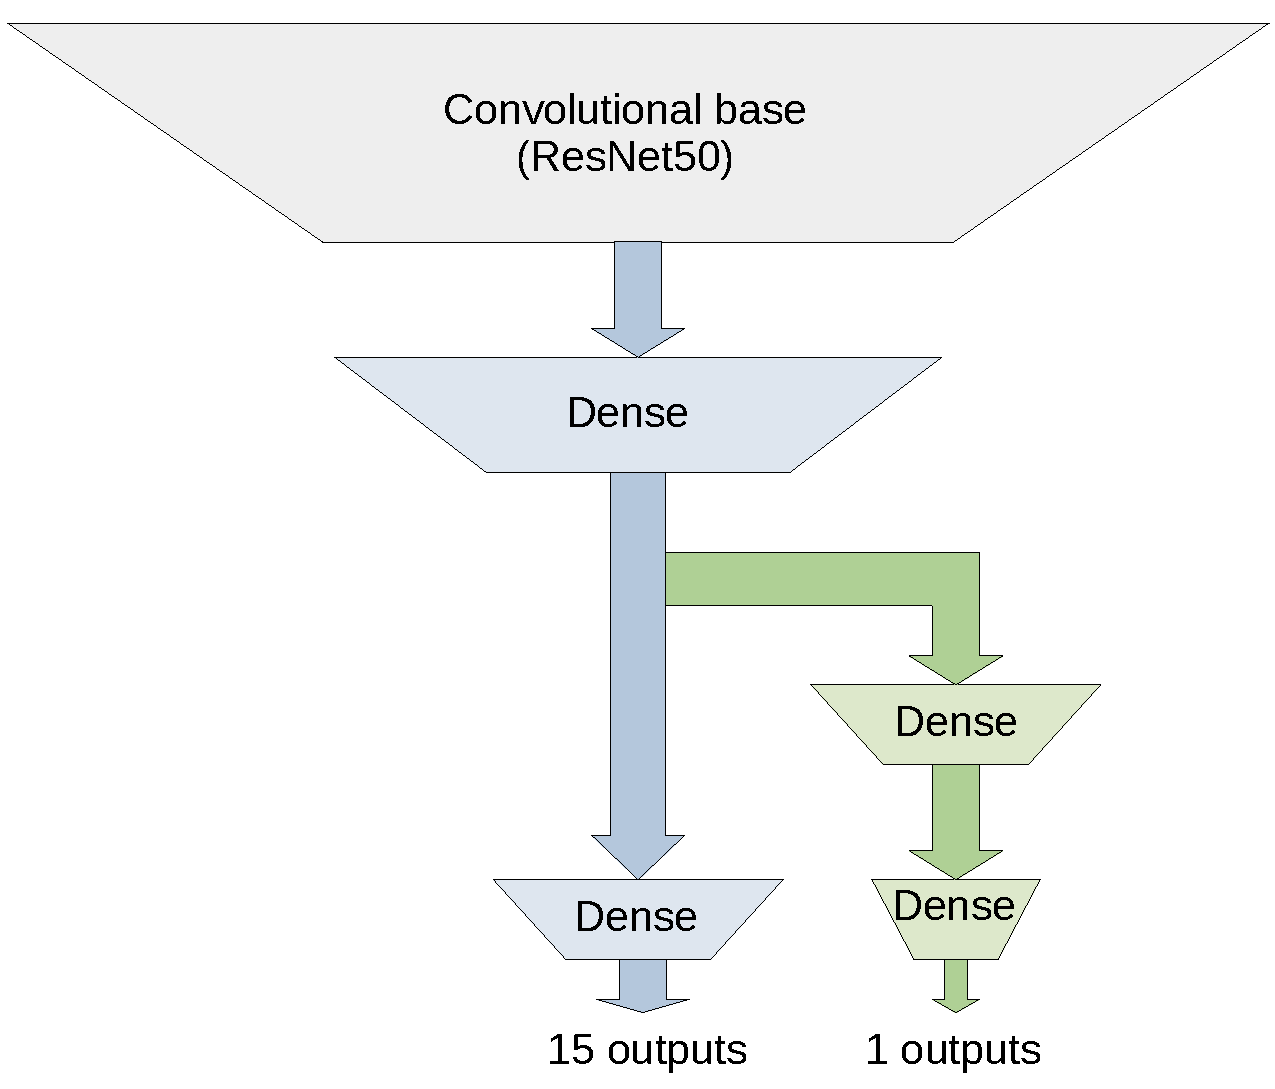
\includegraphics[width=0.5\textwidth]{Chapters/4. ViT-Lung/images/tb_net.pdf}}
\caption{Scheme of the extension of the 15 pathology detector including a new branch for Tuberculosis detection.}
\label{net_tb}
\end{figure}


\subsubsection{Métricas de Evaluación}

Considerando un problema de clasificación binario donde cada radiografia tiene una etiqueta
$y = \{1, 0\}$ con $1$ indicando la presencia del padecimiento en el paciente y $0$ significando
que se encuentra sano, el detector puede tener dos posibles resultados: una detección positiva (P)
para la enfermedad o una detección negativa (N). La tabla \ref{table_cm} muestra la caracterización
de la etiqueta predicha de acuerdo a los valores reales (Ground Truth, GT). Si un paciente enfermo
es correctamente detectado, tenemos un \textit{Verdadero Positivo} (True Positive, TP) y si la
predicción falla, es una \textit{Falso Positivo} (False Negativo, FN). Por otro lado, si una etiqueta
positiva es erroneamente predicha en un paciente saludable entonces tenemos un \textit{Falso Positivo}
(False Positive, FP), y si el paciente saludable es correctamente predicho es un
\textit{Verdadero Negativo} (True Negative, TN). La tabla \ref{table_cm} muestra la \textit{Matiz de
Confusión} con el conteo de cada tipo de predicción en el conjunto de prueba.

\begin{table*}[!ht]
    \centering
    \begin{tabular}{ccccl}
    %\cline{3-4}
    &  & \multicolumn{2}{ c }{Prediction} \\
    %\cline{3-4}
    \multicolumn{1}{c}{}& & Positive & Negative &    \\
    \cline{3-4}
    \multicolumn{1}{c}{\multirow{6}{*}{GT} } &
    \\
    \multicolumn{1}{c}{} & Disease & TP & FN   &  $ \longrightarrow  R = \frac{TP}{TP+FN}$  \\
    \\
    \cline{3-4}
    \multicolumn{1}{ c }{}                    &
    \\
    \multicolumn{1}{c}{} & No-Disease & FP & TN   &  $ \longrightarrow S = \frac{TN}{FP+TN}$   \\
    \\
    \cline{3-4}
    \\
    & & $\downarrow$ & $\downarrow$ & \\
    \multicolumn{1}{c}{} &       & $P = \frac{TP}{FP+FP}$  & $NPV = \frac{TN}{FN+TN}$ &
    \end{tabular}
    \caption{
    Interpretation of the test results (prediction) according to the ground truth (GT). Metrics are calculated as the ratio between the diagonal element and the sum per row or column, as the case may be.  R, recall or sensitivity; S, specificity; P, precision; NPV, negative prediction value}
    \label{table_cm}
\end{table*}

Para este trabajo asumimos que una patología en particular es correctamente detectada si su
correspondiente puntaje en el vector de predicho es más significante que cierto umbral. En particular,
asumimos un umbral igual para todas las patologías de $0.5$. Usando la Matriz de Confusión podemos
definir varias métricas de rendimiento.

\begin{enumerate}
    \item Accuracy ($A$). Esta métrica es quizás la más obvia. Corresponde al razón de los datos
          predichos correctamente sobre el total.
    \begin{equation}
        \label{eq:accuracy}
        A = \frac{TP+TN}{TP+TN+FP+FN}.
    \end{equation}

    \item Recall o Sensibility ($R$). Es la fracción de pacientes con enfermedades conrrectamente
          detectados. Esta metrica también es conocida como Tasa de Verdaderos Positivos (True
          Positive Rate, TPR), la tasa de detecciones correctas.

    \item Specificity ($S$). It is the fraction of patients without the disease that are correctly detected.

    \item False Positive Rate ($FPR$). The rate of false detections of the disease can be calculated with
    \begin{equation}
        \label{eq:FPR}
        FPR = 1- S,
    \end{equation}
    where $S$ is the Specificity.

    \item Precision ($P$). This is the fraction of the predicted as positives that really have the disease, also known as the True Positive Rate ($TPR$).

    \item $F_1$--score ($F_1$). The Recall metric can be bypassed if all the data tested are predicted positive regardless of the evidence. In such a case, $ FN = 0 $  and it result in $ R = 1 $; see the formula for Precision in Table \ref{table_cm}. Similarly, the Precision metric is mocked if all the tested data are predicted as negative. In this other case we will have $FPs = 0$, which implies $P = 1$. Since it is unfeasible to simultaneously cheat both metrics, then an imbalance between them indicates a bias in any of the ways described above. Therefore, it is more informative as a performance measure to use the geometric mean of both metrics.
    \begin{equation}
        \label{eq:f1}
        F_1 = \frac{2\; P \, R}{P + R}.
    \end{equation}

    \item Area Under Curve of Receiver Operator Characteristic (AUC-ROC). The receiver operator characteristic curve is a graph showing the diagnostic capabilities of binary classifiers. We have said that a particular pathology is positively detected if its predicted score is more significant than a given threshold. Then, adjusting such a threshold down allows, in general, to increase the TPR, although the FPR may also be increased. The ROC results of plotting values of TPR vs. FPR  by varying the threshold in the interval $[0,1]$. The AUC corresponds to the area under this ROC curve.

\end{enumerate}
